\documentclass[a4paper,11pt]{article}

% packages
% Eurosymbol
\usepackage{eurosym}
%zum anzeigen von Grafiken
\usepackage{graphicx}
% Sprache Deutsch
\usepackage[english,german]{babel}
% für Referenzen
\usepackage{hyperref}

\author{Baris,Tikir, Leon Dodrimong}
\title{Smart Mirror}

\renewcommand*\contentsname{Inhaltsverzeichnis}
\begin{document}
\maketitle
\newpage
\tableofcontents
\newpage


\section{Grundidee}
\paragraph{Wie wir auf die Idee gekommen sind...}
Auf die eigentliche Idee ist Barsi Tikir eines morgens gekommen als er im Bad stand. Während er sich für den Tag fertig machte und auf seinem Handy noch seine passsende Bahnverbindung raus suchte, dachte er darüber nach, wie praktisch es wäre, wenn man seine Bahnverbindungen nicht mühsam im Handy über die BVG App suchte müsste, sondern diese im irgendwie direkt präsent wäre. Als er darufhin in den Spiegel blickte kam im die Idee.. ein Spiegel  der seine Bahnverbindung anzeigen könnte. Morgens In den Spigel gucken, beim Zähneputzen, Haare machen, usw.... Warum nicht die Zeit auch geich nutzen für ein kleines Update, was in der Welt gerade so passiert oder wann der nächste Bus zur Arbeit fährt. Nach kurzer Recherche fand er auch eine passende Bauanleitung für einen solchen Spiegel. Jedoch gab es neben dem Zusammenbau noch das Problem etwas  sinnvolles auf dem Display anzuzeigen. kleinere Projekt mit Uhrzeit und Wetter gab es bereits, als Beispiele zum nach-programmieren. Aber ein wirkliches System oder fertiges Endprodukt fand er nicht.
\\\
Ein paar Wochen später stieß er auf den Paulaward. Als wir uns trafen, erzählte Baris über die Idee und den Paul Award. Wir fantasierten ein bischen rum und überlegten uns, was denn alles möglich wäre. Zusammen haben wir uns dann rangesetzt und ein Konzept entwickelt, welches möglichst viele Infomationen aus verschiedenen Bereichen anzeigen kann. So entstand die Idee vom "SmartMirror".\\\

\subsection{Spiegel mit integriertem Display}
Ein Spiegel mit integriertem Display ist wohl nichts wirklich neues. Die Idee ist einfach hinter einem Einwegspiegelglass ein Display zu montieren, sodass dieses durch das Glass durch scheint und man dies auf der anderen Seite des Spiegels sehen kann. Von der Anderen Seite wirkt das Galss spiegelnd, wodurch es ganz Normal als Spiegel genutzt werden kann.
\subsection{Gesamtkonzept - eigentliche Idee} 
Unsere eigentliche Idee von uns hinter einen "Spiegel mit integriertem Display" (wird werden ihn im folgenden "SmartMirror" nennen, so wie auch unser Projekt heißt), ist einen System für den SmartMirror zu entwickelt, welches zum einen Benutzerfreundlichkeit(mehr dazu siehe Kapitel \ref{Benutzerfreundlichkeit}) aufweist und zum Anderen mit möglichst vielen Systemen komatibel ist. Wir wollten nicht ein in sich geschlossenes System entwickeln, welches vielleicht gut funktionieren würde, sondern auch ein System, welches bereits vorhandene Dienste nutzen kann. Mehr dazu haben wir im Kapitel \ref{Skalierbarkeit}.
Wir trafen uns meist nach dem Studium und haben uns viele Gedanken darüber gemacht, was der SmartMirror können sollen und über dessen Umsetzung. \\\
Wir stellte einige Grundfunktionen auf die aus unser Sicht wichtig für den SmartMirror wären und welche zusätzlich auch noch sehr praktikabel wären. In diesem Dokument konzentrieren wir uns eher auf die wichtigen Grundfukntionen (Mehr dazu siehe Kapitel \ref{Funktionen} Funktionen).\\\
Danach versuchten wir ein Konzept zu entwickeln, welches allen Anforderungen entspricht. Dabei war es uns sehr wichtig auf den Punkt Skalierbarkeit zu achten.\\\
\begin{figure}[h]
\centering
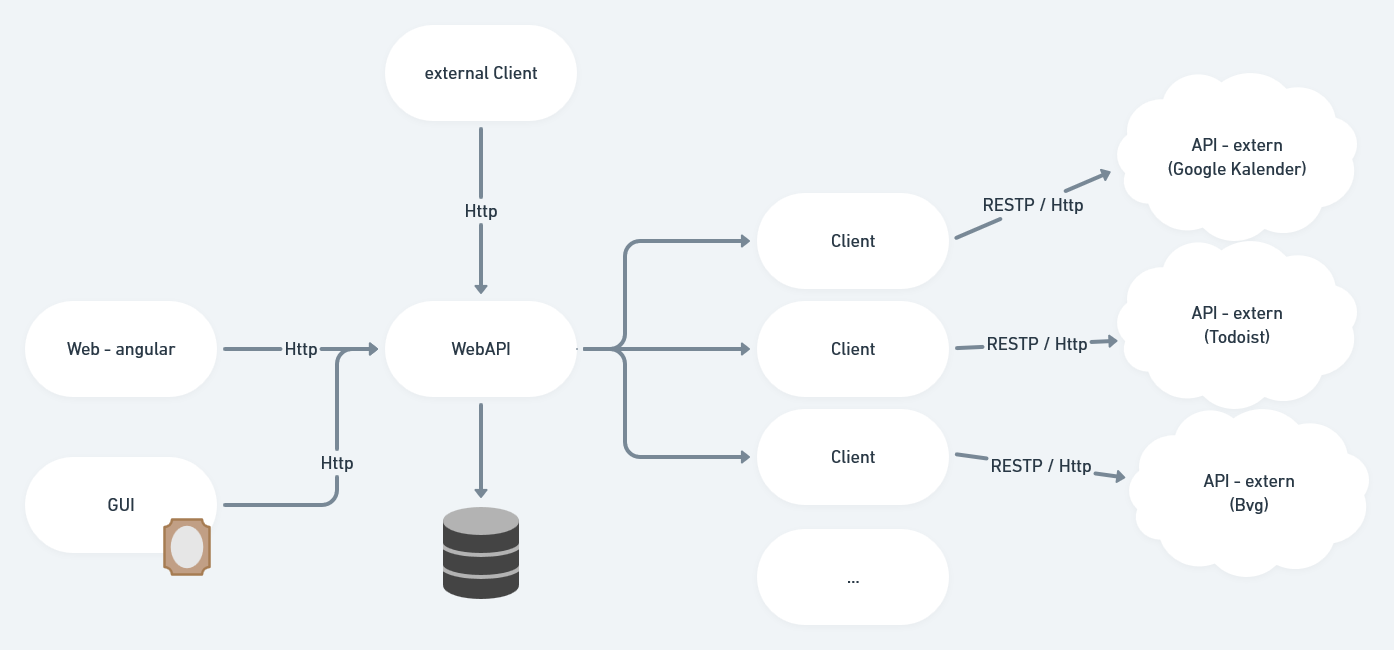
\includegraphics[width=150mm]{pictures/Scalability.png}
\caption{konzeptioneller Aufbau der Software-Komponenten}
\end{figure}\\\
Nach meheren Skizzen und Umgestaltungen kamen wir dann auf diesen Aufbau unserer Software. Auf dem RasperbryPi laufen die folgenden Komponenten: Web - angular, GUI,WebApi, Datenbank und die Clients (mehr zu den einzelnen Komponenten finden sie im Kapitel \ref{Komponenten}). \\\
Die Clients übernehmen die Kommunikation zu den externen Dienst-Anbietern über deren APIs. Die WebAPI organisiert die gesamten anfallenden Daten, wie zum Beispiel: Client-Daten, Benutzerdaten und GUI-Elemente. Auserderm organisiert sie die einzelnen Clients mit deren dazugehörige API und stellt ein eigene API bereit über die Daten abgefragt werden können. Diese API nutzt wiederrum das Frontend, also die GUI Komponente und die Web Komponente. Die GUI ist für die Ansicht auf dem Display hinter dem Glass zuständig. Sie fragt die Daten vom aktuellen Benutzer über die WebAPI ab und formt diese Daten zu einer Ansicht. Die Web Komponente stellt einen Web-Service zur Verfügung, sodass der Benutzer über ein Web-Interface über ein mobiles Endgerät Einstellungen vornehmen kann. Dort kann er Einstllungen bezüglich verschiedener Benutzerkonten und deren Dienste machen. Diese API kann natürlich auch von externen Clients benutzt werden, um zum Beispiel mit eigene SmartHome Produkte mit dem SmartMirror zu interagieren oder den SmartMirror zu steuern.\\\

Um den SmartMirror (RaspberryPi) ins eigene WLAN zu bringen haben wir uns folgende Methodik überlegt. Der RaspberryPi stellt über den integrierten Wifi-chip ein eigenes WLAN zur Verfügung. In dieses muss sich der Benutzer zur Konfiguration einwählen. über ein kleines Web-Interface soll er dann sein WLAN auswählen und das Passwort eingeben oder den SmartMirror über den eigenen WLAN Router freischalten.

\paragraph{Clients}
Die Clients, wobei jeder auf eine spezifische externe API ausgreichtet ist, übernehemen die Kommunikationion zu diesen. Sie kümmern sich um die Authorisierung, Datenabfrage und stellen der WebAPI bestimmte einheitliche Funktionen bereit. Jeder Client muss diese implementieren. Zusätzlich ist der Aufbau der Daten, die zwischen der WebAPI und den Clients übertragen werden, vereinheitlicht und fest definiert. Diese vereinheitlichten Funktionen und Datenmodelle sind in von uns definierten Interfaces beschrieben. Ein Client muss sich an die vorgebenen Funktionen und Datenmodelle halten. Dabei haben wir geguckt, welche Funktionen essentiell wichtig für die Kommunikation sind und wie wir die Daten optimal strukturieren können. (einige Funktionen um nicht zu sehr ins Detail zu gehen zb.: getData(Options):Data, welche Daten von der API und den Bedingungen abfragt; getOptions():Options, welche die Verfügbaren Optionen abfragt; setToken(string):bool, welche den Authorisierungstoken für den jeweiligen Client setzt). Wenn eine neue externe API bereitgestellt werden soll, muss lediglich ein Client programmiert werden, welcher die vorgeschriebenen Funktionen und Datenmodelle implementiert (Interfaces) und die jeweiligen Http-Requests für die API beinhaltet. So kann zu jeder API unter berücksichtigung der Interfaces ein passender Client programmiert werden.\\\
\paragraph{WebAPI}
Die WebAPI übernimmt die 


\subsubsection{Benutzerfreundlichkeit}\label{Benutzerfreundlichkeit}
Die eigentliche Idee dabei ist den Spiegel nicht einfach nur spiegeln zu lassen oder die Uhrzeit anzeigen zu lassen, sondern ihn "smart" zu machen, sodass man ihn praktischen und effizient Nutzen kann. Zudem war uns auch wichtig, dass es \textbf{Benutzerfreundlich} ist, da nicht jeder das Know-How hat sich einen Spiegel für seine Eigenen Bedrüfnisse zusammen zu bauen bzw. zu programmieren. Er sollte einfach und verständlich für jeden sein. Deshalb haben wir auch die in das Konzept die Web Komponente eingefügt und die GUI leicht erweiterbar gestaltet.

\subsubsection{Skalierbarkeit}\label{Skalierbarkeit}
Der SmartMirror ist nicht nur Benutzerfreundlich, sondern ist auch in vielen Richtungen skalierbar.
Wie schon erwähnt, wollten wir die bereits bestehenden Dienste Nutzen. Zum Beispiel hat man seine Kalendereinträge bereits im Google-Kalender eingetragen und hat keine Lust als Kunde alle Daten auf den Kalender des SmartMirrors zu übertragen. Es wäre für den Benutzer leichter auf diese Daten zuzugreifen. \\\
Viele Anbieter von Diensten stellen über das Http-Protokoll API Funktionen für Ihren Dienst bereit. Diese API's nutzt der SmartMirror, um dann die Daten vom dem jeweiligem Dienst abfragen zu können. Dieses Abfragen geschieht in der Client Komponente, auf welche wir näher im Kapitel \ref{Clients} Clients eingehen werden. Dadurch ist das System erweiterbar und hilft sogar beim Vernetzen von anderen Diensten.\\\
Neben der Erweiterbarkeit haben wir auch daran gedacht, eine eigene Schnittstelle zu definieren, sodass andere SmartHome-Produkte sich an den SmartMirror vernetzen können. Diese können dann wie die GUI und Web Komponente, Daten vom SmartMirror abfragen oder senden, sodass es zum Beispiel auch denkbar wäre mehrere SmartHome-Produkte so miteinander zu vernetzen, dass der SmartMirror die Basis bildet.\\\
Im Sinne von Smart Home und Industrie 4.0






\section{Aufbau}
Dem Aufbau der Software haben wir aufgrund der Vielfalt ein eigenes Kapitel gewidmet. (\ref{Software})
\subsection{Hardware - Spiegel}
\begin{figure}[h]
\centering
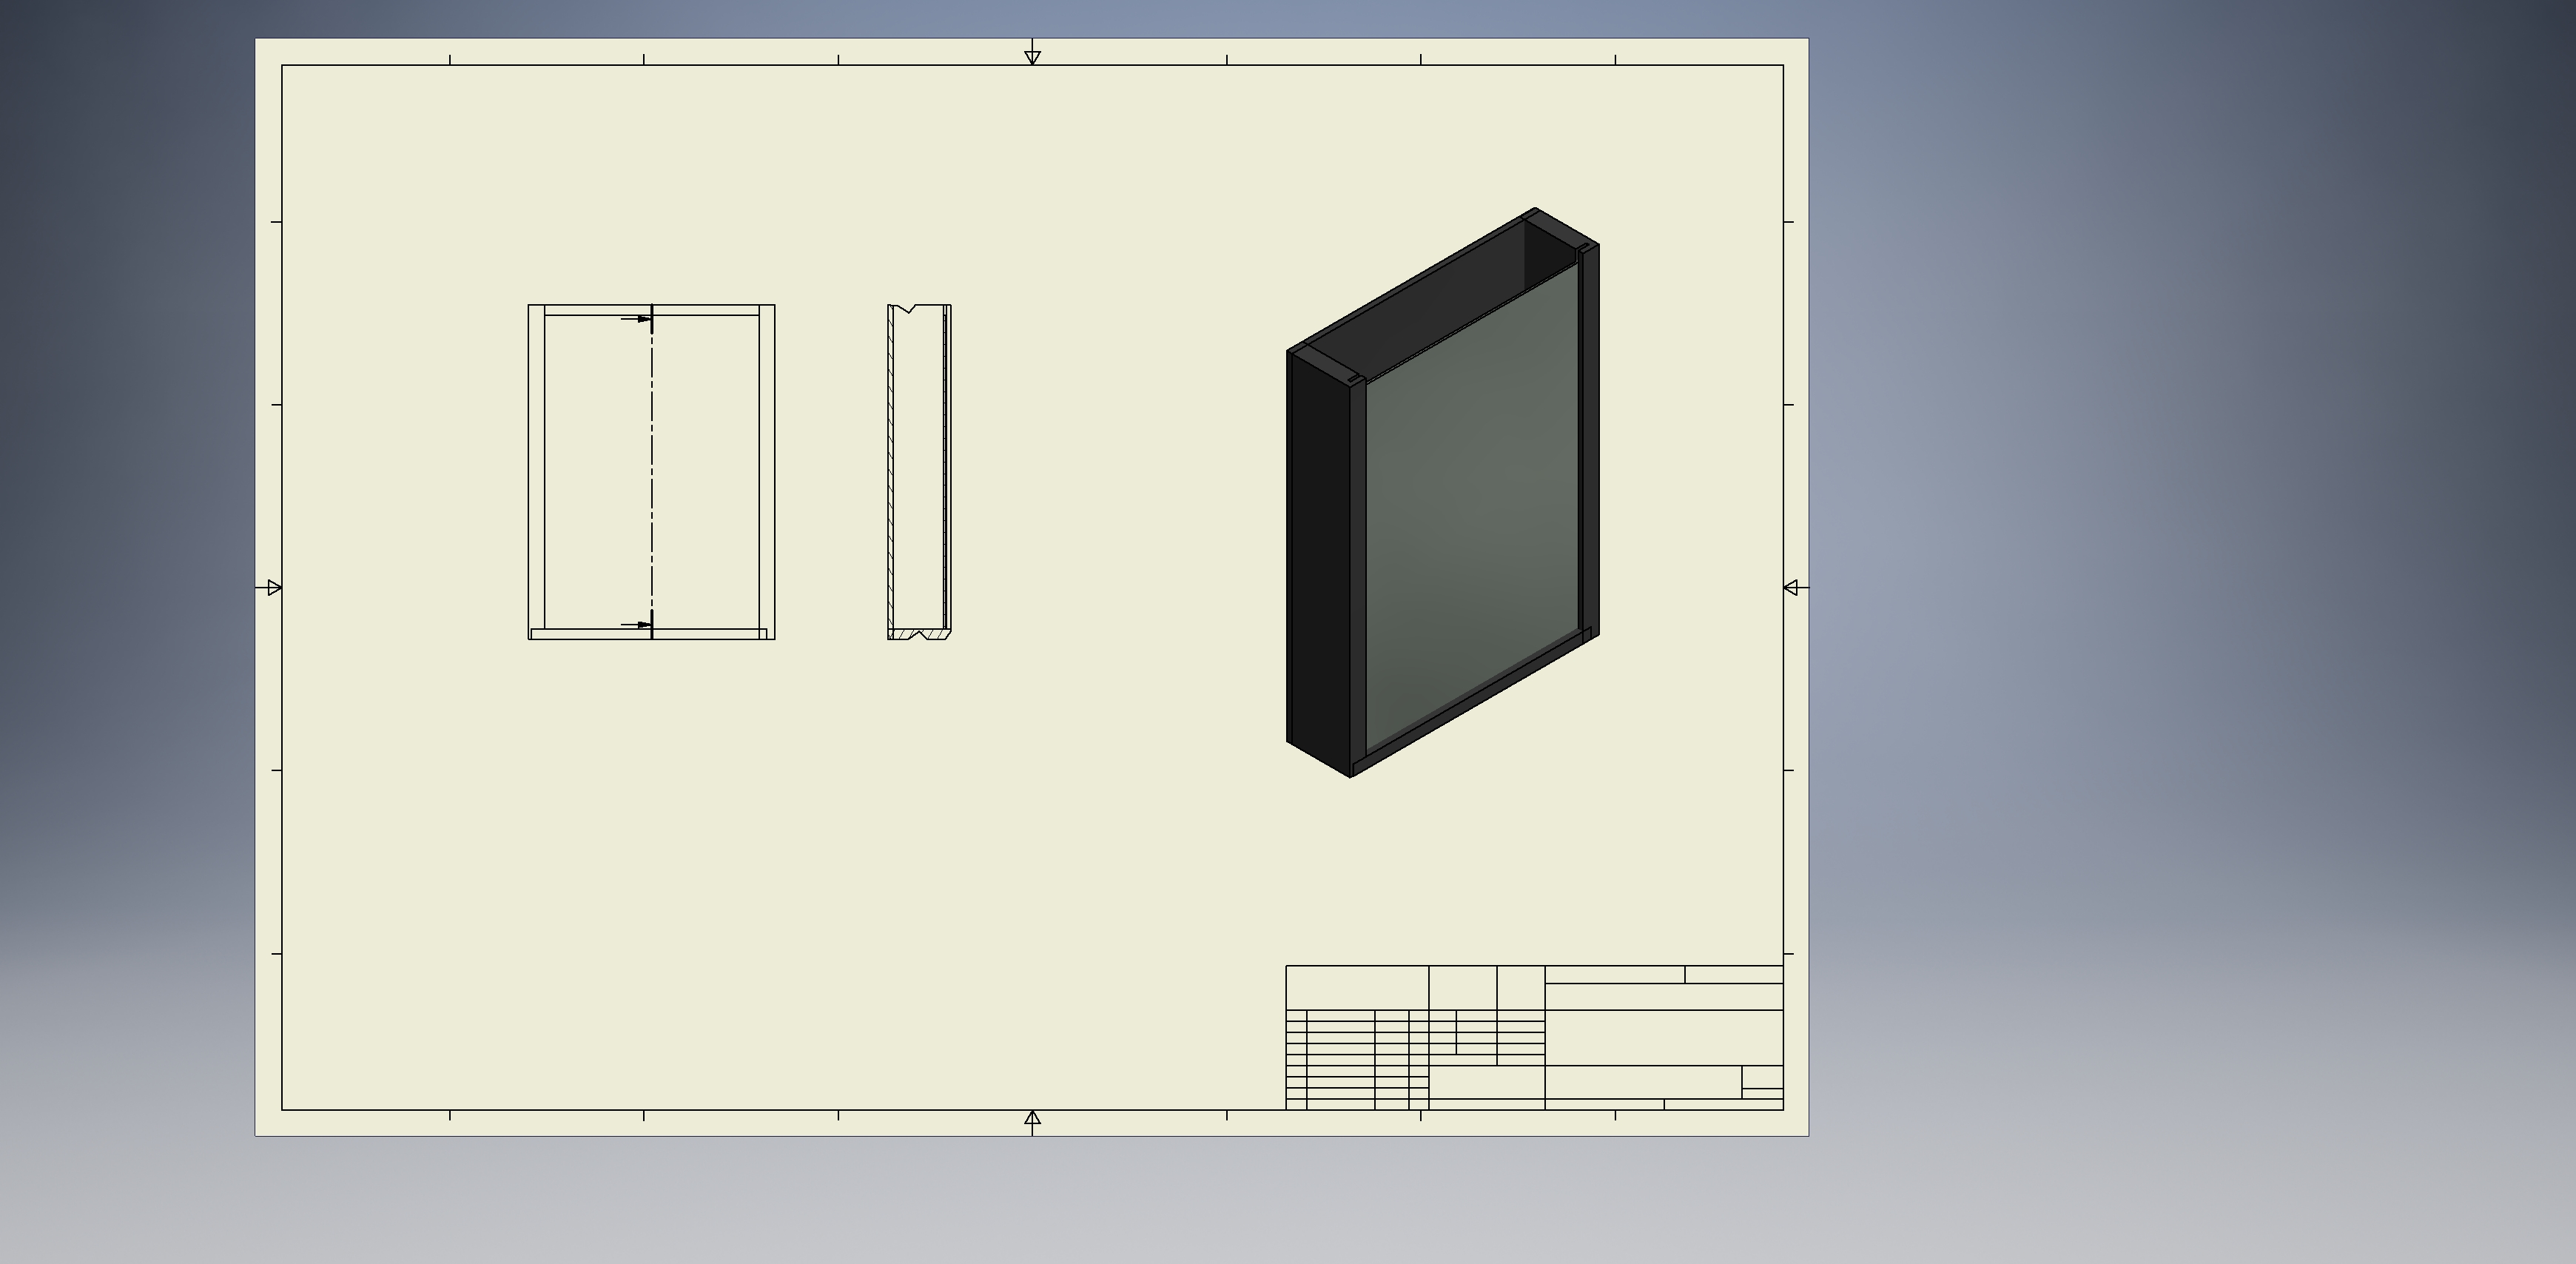
\includegraphics[width=150mm]{pictures/SmartMirror-Konstruktion.jpg}
\caption{konzeptioneller Aufbau der Software-Komponenten}
\end{figure}
Die folgende Zeichnung stellt die Konstruktion, der Rahmen Elemente sowie dem Spiegelglas, dar. Beim Querschnitt, in der Zeichnung oben links dargestellt, wird ersichtlich, dass zwischen dem Spiegelglas und der Spiegelrückenwand eine Lücke von ca. 10cm ist. Dort wird sich im Nachhinein der Monitor/Display und der Raspberry Pi befinden. In der Bodenplatte des Spiegels sind Bohrungen versehen, die für die Kabeldurchführungen vorgesehen sind. Die Öffnung oben ist dafür vorgesehen, dass das Rausnehmen des Spiegelglases und der ganzen Technik vereinfacht wird.\\\
Für eine Montage des SmartMirrors im Badezimmer wäre noch ein extra angefertigtes Gehäuse, für die Technik, notwendig um Schäden, die durch Feuchtigkeit und etc. entstehen, zu vermeiden.
\subsection{Materialien}
Der Spiegel besteht aus einem Einwegspiegelglass, welches von einer Seite spiegelt und von der anderen Seite reflektiert. Außerdem haben wir einen Holzrahmen, welcher aus Fassung für das Spiegelglass dient, genutzt. Für die Technik haben wir ein Display für die Anzeigen , ein RasperryPi für die Steuerung und die nötigen Verbindungskabel, wie Spannungsversorgung und Videokabel (HDMI) zur Übertragung der Videosignals zum Display, eingesetzt.\\\
Für die optinalen Erweiterungen würde man je nachdem welches Feature gewünscht ist, noch eine Picamera (für Facerecognition), RasperryPi Bewegungssensor (Bewegungserkennung)\footnote{\textit{ Raspberry Pi Infrarot Bewegungsmelder:} https://www.reichelt.de/raspberry-pi-infrarot-bewegungsmelder-hc-sr501-rpi-hc-sr501-p224216.html?\&nbc=1}, Gesture Sensor (Gestiksteuerung)\footnote{\textit{3D Gesture Tracking Shield for Raspberry Pi:}  http://wiki.seeedstudio.com/3D-Gesture-Tracking-Shield-for-Raspberry-Pi-MGC3130/} oder ein kleines Mikrophone zur Sprachsteuerung \footnote{\textit{Ansteckmikrofon über Klinke:} https://www.amazon.de/dp/B073GJQKL1/ref=psdc\_1384055031\_t1\_B07WQFNVVQ}

\paragraph{Kosten}
Da der SmartMirror für Jederman sein soll, darf dieser auch nicht das Budget eines Einzelnen sprengen. Daher hatten wir auch im Hinterkopf, dass die Koponenten nicht zu teuern sein dürfen.\\\
\begin{itemize}
\item Der Raspberry Pi kostet ca. \EUR{40} 
\item das Spiegelglas, was wir verwendet haben ist etwas teurer und zwar beträgt der Preis ca. \EUR{80}, da es ein Spionspiegel ist und extra für solch einen Zweck konstruiert wurde. Nur eine Seite des Glases kann spiegeln, was die Darstellung des Monitors unter dem Spiegelglas verschönert. Das Spiegelglas kann auch für deutlich billiger besorgt werden, in dem man nur eine Spiegel-Folie, die ca. \EUR{10} kostet, direkt auf den Monitor angebracht werden kann.
\item Das Dispaly mit dem zugehörigen Controller kostet mit Kabeln ca. \EUR{50}
\item Spiegel Rahmen und Material kostet ca. \EUR{10}-\EUR{20}
\item Gesamtpreis wäre zwischen eine Preisspanne von \EUR{120}-\EUR{190}, je nach Qualtitätswahl und Anforderungen
\end{itemize}
Wenn man überlegt, dass ein Normaler Spiegel ca. \EUR{80}-\EUR{100} kostet, recht preiswert ist.

\section{Software}\label{Software}
\subsection{Prerequisites}
\begin{itemize}
\item Node.js (Javascript runtime)
\item Angular
\item IDE (Visual Studio Code)
\item Datenbank (MariaDb)
\end{itemize}

\subsection{Frontend - SmartMirrorWeb}
\begin{figure}[h]
\centering
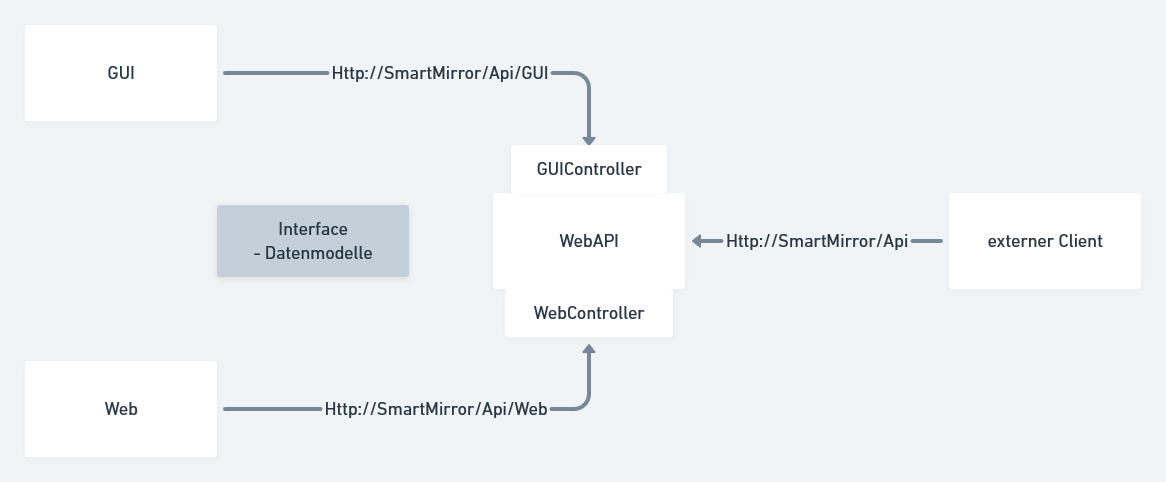
\includegraphics[width=120mm]{pictures/Frontend2.png}
\caption{konzeptioneller Aufbau der Software-Komponenten}
\end{figure}
Unser Frontend besteht aus einer GUI- und Web-Komponente. Die GUI ist dafür zuständig die Daten, die auf dem Spiegel angeziegt werden zu verwalten und entsprechend auf dem Display hinter dem Spiegel auszugeben. Die Web-Komponente hingegen stellt dem Benutzer über das Web Frontend Funkionalität zur Verwaltung der Benutzerdaten, sowieso zur Verwlatung der Inhalte der GUI, zur Verfügung. Dies kann über ein mobiles Endgerät erreicht werden (Beispielsweise einem im Netzwerk befindlichen Computer oder SmartPhone).\\\
Das Frontend übernimmt folgende Hauptaufgaben:
\begin{itemize}
\item Anzeigen der Daten
\item Eingabemöglichkeiten anbieten
\begin{itemize}
\item GUI: Face Recognition, Voice Control, Motion Control
\item Web: Web-Formulare, Buttons
\end{itemize}
\item Datenaustausch mit Backend
\end{itemize}



\begin{itemize}
\item Daten vom Backend (SmartMirror.WebApi) anfragen
\begin{itemize}
\item alle möglichen Dienste (Widgets)
\item vom User angemeldeten Dienste
\end{itemize}
\item Daten senden
\begin{itemize}
\item Dienst aktivieren/ deaktivieren
\item Benutzereingaben zur Erstellung eines neuen Benutzers
\end{itemize}
\item User zur Anmeldung von weiteren externen Diensten, zur jeweiligen Website weiterleiten\footnote{zum Beispiel: wenn der User den neuen Dienst Google Kalender für sich registrieren möchte, muss er sich auf der Website von Google Kalender anmelden um sich zu zertifizieren. Diese sendet dann die zur Authentifizierung notwendigen Credentials, welche vom Backend gespeichert werden müssen }
\end{itemize} 

\subsection{Backend - SmartMirror.WebApi}
Das Backend besteht aus einer eigens Entwickelten Web API, welche zum einen die Anfragen und Daten vom Frontend (SmartMirror.Web) entgegennimmt und bearbeitet, und zum anderen den Datenaustausch mit der eigenen Datenbank und Kommunikation mit den externen API kommuniziert.\\\
Das Backend besteht aus einen Client-Server. Zum einen stellt er als Server eine eigene API dar, welche vom Frontend oer externen Clients genutzt werden kann. Zum anderen fungiert dieser auch als Client und nutzt die externen API Schnittstellen von Drittanbietern. AUßerdem besitzt dieser eine extra Komponente, welche auf die interne Datenbank zugreift\\\
Mehr dazu befindet sich im folgenden Kapite \ref{Komponenten}



\subsection{Komponenten}\label{Komponenten}
Für das Komponentendiagramm siehe \ref{Komponentendiagramm}.
\subsubsection{Clients}\label{Clients}
Da der Smart Mirror möglichst viele externe Features verbinden soll, muss die Schnittstelle zu diesen gut strukturiert werden. Daher haben wir uns dazu entschieden, dass jede externe Kommunikation ihre eigene Komponente bekommet, welche bestimmte Standards (Interfaces) bedient.\\\
Die Clients, wobei jeder auf eine spezifische externe API ausgreichtet ist, übernehemen die Kommunikationion zu diesen. Sie kümmern sich um die Authorisierung, Datenabfrage und stellen der WebAPI bestimmte einheitliche Funktionen bereit. Jeder Client muss diese implementieren. Zusätzlich ist der Aufbau der Daten, die zwischen der WebAPI und den Clients übertragen werden, vereinheitlicht und fest definiert.\\\
Diese vereinheitlichten Funktionen und Datenmodelle sind in von uns definierten Interfaces beschrieben. Ein Client muss sich an die vorgebenen Funktionen und Datenmodelle halten. Dabei haben wir geguckt, welche Funktionen essentiell wichtig für die Kommunikation sind und wie wir die Daten optimal strukturieren können. (einige Funktionen um nicht zu sehr ins Detail zu gehen zb.: getData(Options):Data, welche Daten von der API und den Bedingungen abfragt; getOptions():Options, welche die Verfügbaren Optionen abfragt; setToken(string):bool, welche den Authorisierungstoken für den jeweiligen Client setzt).\\\
Wenn eine neue externe API bereitgestellt werden soll, muss lediglich ein Client programmiert werden, welcher die vorgeschriebenen Funktionen und Datenmodelle implementiert (Interfaces) und die jeweiligen Http-Requests für die API beinhaltet. So kann zu jeder API unter berücksichtigung der Standards ein passender Client programmiert werden. Anschließend muss dieser nur noch der WebAPI bekannt gemacht werden, indem der Client in eine interne Liste von allen möglichen externen Diensten eingetragen wird.\\\

\subsubsection{Database}
\begin{figure}[h]
\centering
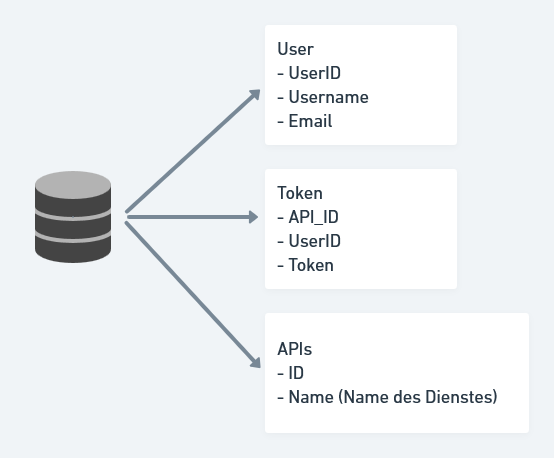
\includegraphics[width=80mm]{pictures/Database.png}
\caption{Aufbau der Datenbank}
\end{figure}
Die Datenbank ist die Hauptspeicherkomponente des SmartMirrors. Sie speichert sämtliche Daten. Die Daten haben wir vorerst in drei Tabellen aufgeteilt.\\\
Die Tabelle \dq User \dq speichert Daten in Bezug auf Benutzerprofile, wie zum Beispiel den Benutzernamen mit Email und ordnet jedem Benutzerkonto eine eindeutige ID zu, sodass er darüber authentifiziert werden kann\\\
In \dq Token \dq werden die Authentifizeriungstoken in Bezug auf die entsprechende API vom entsprechendem Benutzerprofil.\\\
In der dritten Tabelle \dq APIs\dq werden die verschiedenen externen APIs aufgelistet mit entsprechendem Namen. Jeder wird auch hier eine eigene ID zugewiesen. Dies dient dem ClientManager zur Organisation für die Clients und zur Abfrage der entsprechenden Token.\\\
In Zukunft werden wohl hier noch weitere Daten, wie zum Beispiel, Layouts in Bezug auf das Benutzerprofil und Zustände der APIs eines Benutzerprofils (aktiviert, deaktiviert), anfallen.

\subsubsection{WebAPI}
\begin{figure}[h]
\centering
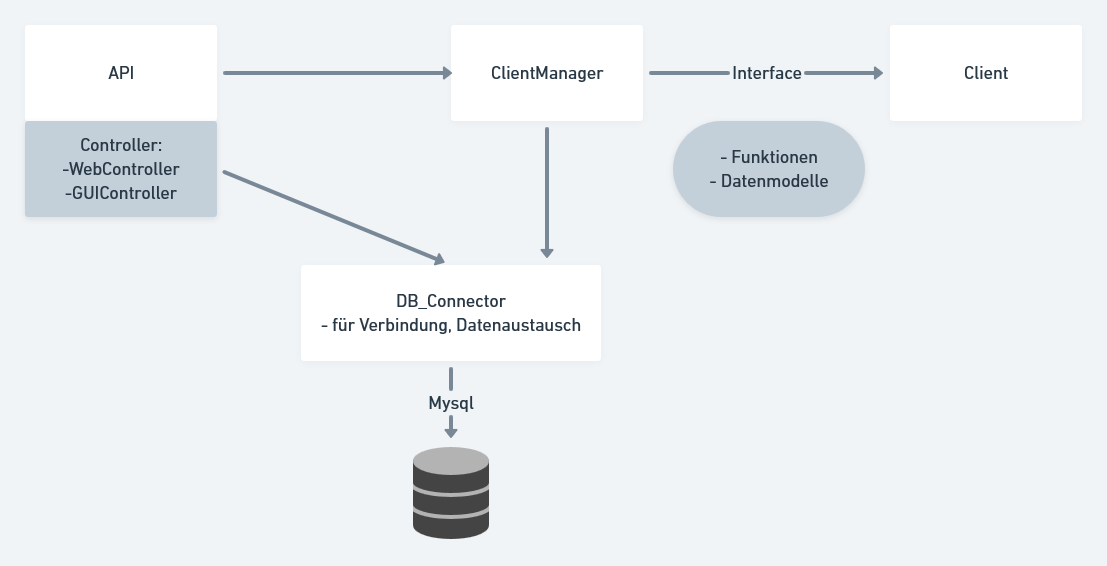
\includegraphics[width=120mm]{pictures/WebAPI.png}
\caption{Komponenten der WebAPI}
\end{figure}
Die WebAPI besteht aus drei Hauptkomponenten. Zum einen der eigentlichen REST API Schnittstelle, einer Komponente zur Datenbank Verbindung und einer Client Komopente. Die API stellt über eine REST API (Http-Protokoll) Funktionen und Daten zur Verfügung, die die verschiedenen Komponenten verwenden (GUI,Web und externe Clients). Die Funktionen haben wir in zwei Bereiche aufgeteilt. Zum Einen Funktionen, die hauptsächlich von der Web Komponente genutzt werden im WebController, und zum Anderen Funktionalitäten, die hauptsächlich die GUI Komponente Nutzt im GUIController. C\# arbeitet mit Controller, welche über verschiedene URLs angesprochen werden können. Die API ist der wichtigste Kommunikationspunkt für das Frontend. Sie greift außerdem auf die anderen beiden Komponenten (DB\_Connector und Client/Clientmanager) zu.\\\
Die DB\_connector stellt die Verbindung zur Datenbank her und sendet SQL Requests um Daten auszutauschen.\\\
Der Clientmanager greift auf die den DB\_Connector zu, um Daten, wie Token für die Authorisierung, abzufragen. Die Hauptaufgabe vom ClientManager ist jedoch, dass organisieren der einzelnen Clients. Da für jede externe API ein bestimmter Client existiert, muss der ClientManager sich merken welcher Client mit welcher externen API (Identifizierung der verschiedenen externen APIs erfolgt über die Datenbank) asoziiert wird. Er nimmt die Anfragen von der API, holt sich den entsprechenden Authorisierungstoken aus der Datenbank und leitet diese Anfrage an den entsprechenden Client weiter. Da jeder Client die Funktionen und Datenmodelle,welche in den Interfaces definiert sind, implementiert, kann der ClientManager die entsprechnende Funktion beim Client aufrufen und bekommt Daten in einem definierten Format zurück. Diese Daten werden dann wieder zurück über die API an den anfragenden Client gesendet (meist GUI- oder Web-Komponente).


\subsubsection{GUI}
Die digitale Darstellung, aller Module die zuvor auf der Website konfiguriert wurden, auf dem Spiegel wird durch unsere eigene GUI - Applikation (\dq Graphical User Interface\dq ) ausgeführt. Diese wurde in der Programmiersprache C\# geschrieben, welches uns die simple Erstellung einer Desktop Applikation ermöglichte und uns zudem auch aus dem Studium bekannt ist. 
Das Ziel war es ein kompatibles System aufzubauen. Deshalb sollte die Applikation Betriebssystem unabhänig sein, dass heißt es sollte auf jedem Betriebssysteme mit gleicher Performance laufen können. Die Wahl mit C\# und .NET hat diese Entscheidung für uns schwer getan, da das .NET Framework und .NET Core ihre Windows Desktop Applikationen eher für \dq Windows-only\dq , von Microsoft, konzipiert wurden. Das Betriebssystem auf dem Raspberry Pi ist \dq Raspbian\dq  und basiert auf den Linux Kernel. Das Problem konnten wir mit einigen zusätzlichen Erweiterungen beheben. Um eine Kompatibilität unserer GUI-Applikation mit Linux herstellen zu können, mussten wir zusätzliche Framework Installationen auf den Raspberry Pi durchführen. 
Eine Lösung wäre das \dq Avalonia-Framework\dq , welches die Entwicklung von Desktop Applikationen unter .NET Core in der Programmiersprache C\# ermöglicht. Damit könnte man schon von Beginn an die Applikation für Linux entwickeln. Diese Lösungsmöglichkeit wird auch auf unser GUI-Projekt (\dq SmartMirror.GUI\dq , im GitHub Repository zu finden) angewandt. 
Für Universelle Windows Systeme haben wir die \dq SmartMirror.GUI\_UWP\dq  entwickelt. Die Benutzeroberfläche ist identisch wie die SmartMirror.GUI, die selben Funktionalitäten werden unterstützt nur für verschiedene Systeme.

\subsubsection{Web}
Wir haben unser Frontend mithilfe von Angular 9 entwickelt. Für uns war dies eine Neue Erfahrung, da wir noch nie zuvor damit gearbeitet haben.


\section{Funktionen}\label{Funktionen}
\subsection{Grundfunktionen}
\begin{itemize}
\item Daten von externen API's abfragen
\item Daten von externen API's anzeigen (Widgets)
\item Einstellungen über ein Web Frontend vornhemen
\item Schnittstelle für andere Erweiterungen (externe Clients)
\item ...und natürlich auch die Grundfunktion spiegeln nicht vergessen
\end{itemize}

%
%\begin{itemize}
%\item Google Kalender
%\item Todoist
%\item BVG
%\item Wetter
%\end{itemize}
\subsection{Extras}
\begin{itemize}
\item Face Recognition
\item Voice Control
\item Bewegungssensor
\item Motion Control
\end{itemize}

\subsection{Face Recognition}
Ein SmartMirror mit einem einzigen Ansichts Fenster und auch nur einem Kalendar wäre nicht das optimalste in jedem Haushalt, denn jedes Familienmitglied oder jeder Mitbewohner hat seine eigenen Termine und Kalendareinträge. Eine mögliche Lösung wäre das jeder seinen eigenen SmartMirror besitzt, es wäre jedoch nicht effizienteste und effektivste Lösung. Daher wäre die beste Lösung die "Face-Recognition". Dieser hat die Funktionalität, mithilfe von Machine Learning sich das Gesicht zu merken und es auch wiederzuerkennen. Es könnte dadurch für jede Person im Haushalt ein Profil angelegt werden, und alles was an Modulen und Einstellungen getätigt wird innerhalb dieses Profiles zuspeichern. Je nachdem wer dann vor dem Spiegel steht, dessen Profil, die jeweiligen Module werden, geladen und im Spiegel dargestellt, als Beispiel der Kalendar der jeweiligen Person. 
\begin{figure}
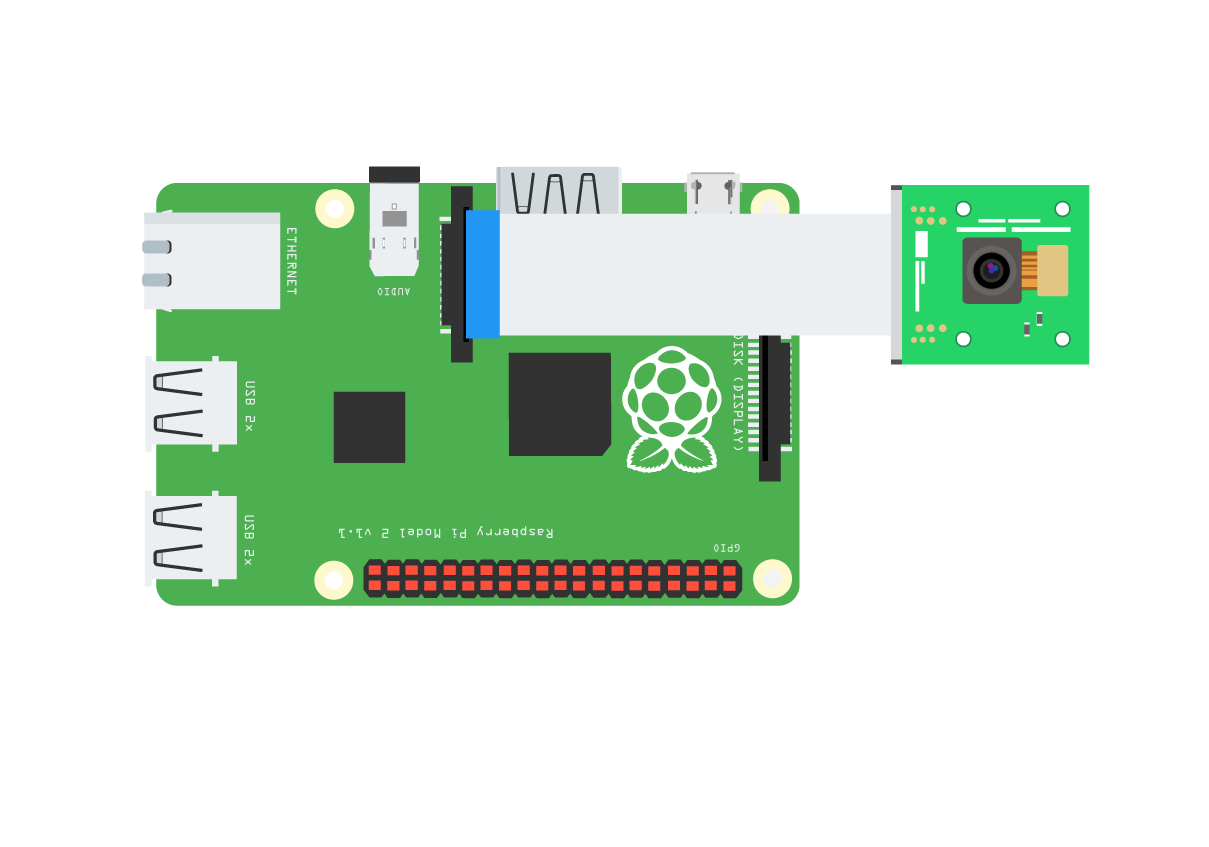
\includegraphics[width=100mm]{pictures/raspberry-pi-camera-2.png}
\caption{Raspberry-pi Kamera}
\end{figure}
\subsection{Voice Control}
Was gebe es noch cooleres als ein Voice Control System im Spiegel? Während man am Haare fönen ist oder der Bart mal wieder rasiert werden muss und nebenbei Aufgaben, wie Kalendar Einträge \& Todo-Aufgaben hinzufügen zu lassen oder auch die Abfahrten der lokalen Öffentlichen Verkehrsmittel, wie Bus und Bahn,  abfragen kann, sowie jegliche Staumeldungen auf der Autobahn, mit nur einem Satz erledigt werden können. Als Hardware wird lediglich ein Mikrof und ein Latusprecher benötigt.

\subsection{Bewgungssensor}
Um unseren SmartMirror möglichst effizient zu gestalten wäre die Verwendung eines Bewegungssensor sehr angebracht. Es sollte so funktionieren, dass sobald jemand vor dem Spiegel steht, der Spiegel aus dem Stand-By Modus zum Aktiven Modus wechselt. Somit wäre der Spiegel nicht die ganze Zeit über an und würde den Stromverbrauch deutlich senken. Der wäre an Bodenplatte des Spiegels zu befestigen. 
\begin{figure}
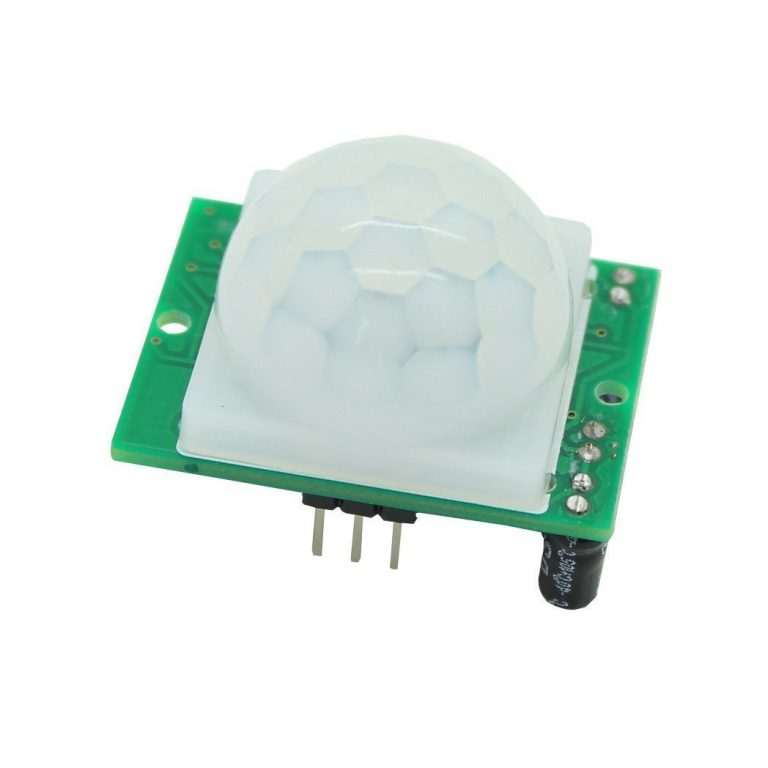
\includegraphics[width=50mm]{pictures/Bewegungssensor.jpg}
\caption{Bewegungssensor}
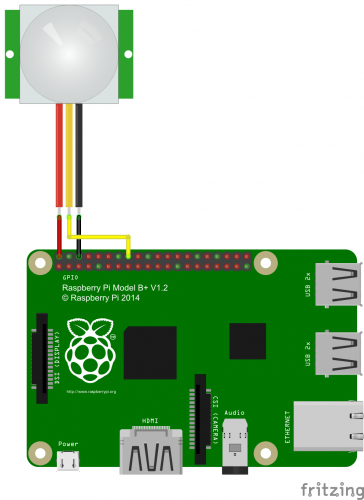
\includegraphics[width=80mm]{pictures/Bewegungssensor_Plan.png}
\caption{Schaltplan}
\end{figure}
\subsection{Motion Control}
Um mehrere Ansichts Fenster auf dem SmartMirror zu besitzen und ziwschen denen auch navigieren zu können, wäre ein Motion-Control erforderlich. Dieser ermöglicht mit Gestiken, wie mit der Hand zur Seite wischen um die Seite zu wechseln, zu navigieren. Diese wären aber natürlich selber programmier- und konfigurierbar. 
Als Hardware für dieses Konzept wäre ein Entfernungsmessungssensor, wie der von Sharp der "Sharp Reflektierender Sensor- GP2Y0A21YK0F"*, ein Analog zu Digital Konverter, wie der von Microchip "8-Channel A/D Converter - MCP3008"*, und ein Breadboard erforderlich.
Der Entfernungsmessungssensor kann die Entfernung von Objekten, mithilfe von Infrarotstrahlen, die am Objekt reflektiert werden, ermitteln. Der Konverter wird benötigt, da der Raspberry Pi nur Digitale Ein- und Ausgänge besitzt und der Entfernungsmessungssensor Analogen Ausgänge besitzt. Das Breadboard wäre dafür da, um den Raspberry Pi und den Sensor über den Konverter zu verbinden.
\begin{figure}
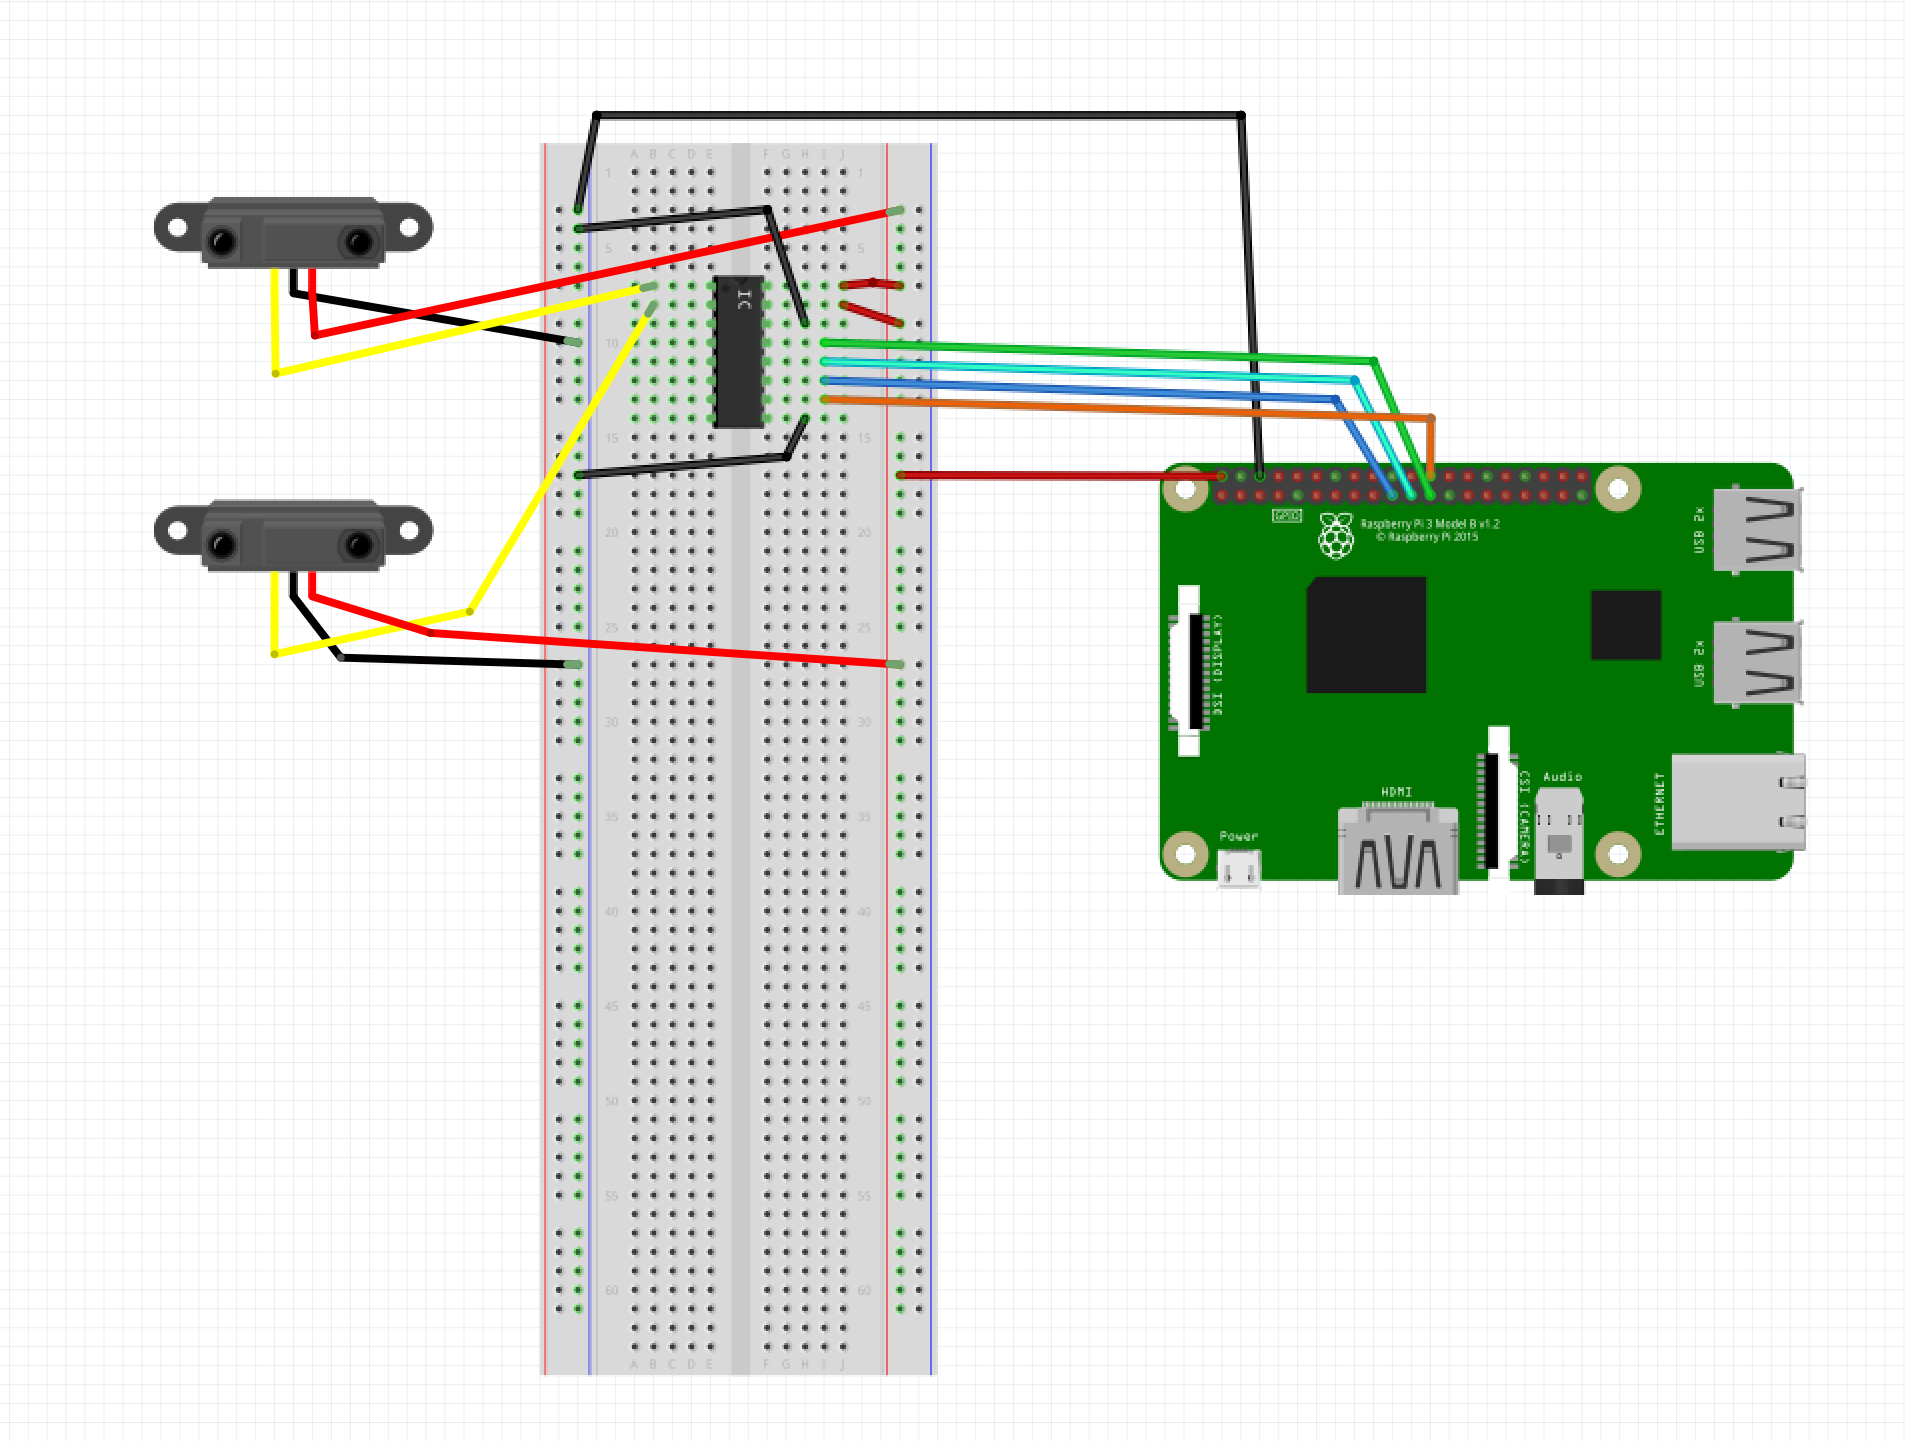
\includegraphics[width=100mm]{pictures/Motion-Control_Plan.PNG}
\caption{Schaltplan}
\end{figure}

\section{Tests}
Wir haben bis zum letzten Entwicklungsstand vor der Abgabe jede Komponente Einzeln getestet. Die Funktionen die wir bis zu dem Zeitpunkt implementiert haben, funktionierten. Das Zusammenspiel einzelner Komponenten wurde ebenfalls getestet durch extra angefertigte Test. So haben wir zu Beispiel ein Test Projekt angelegt in dem wir den im Frontend benutzten API Client für unsere WebAPI testen konnten, indem wir die Datenbank mit Beispiel Daten belegten und dann einige Testanfragen laufen ließen.\\\
Wir verbrachten viel Zeit mit der Konzeptionierung, dem Entwurf und vorallem mit der Informationsbeschaffung, da wir vor diesem Projekt mit vielen Techniken noch keine Erfahrungen gemacht haben und uns einiges erst noch beibringen mussten.\\\
Leider konnte der komplette SmartMirror nicht komplett getestet werden, da uns einfach gesagt die Zeit fehlte. Wir werden das Projekt jedoch in Zukunft fortsetzen.
\\\
Das Projekt befinden sich auf \textbf{Github} in folgendem Repository: 

https://github.com/brstkr/SmartMirror.git\\\

\section{Über uns}
Wir sind zwei Studenten, Baris Tikir und Leon Dodrimong, von der HTW - Hochschule für Technik und Wirtschaft Berlin aus dem Fachbereich der Ingenieurwissenschaften und Technik. Wir befinden uns zur Zeit im dritten Semester. Wir beiden lernten uns über das Studium kennen, welches wir beide im Wintersemester 2018/19 starteten.

\newpage{}
\section{Anhang}
\subsection{Diagramme}
\label{UseCase}
\begin{figure}[h]
\centering
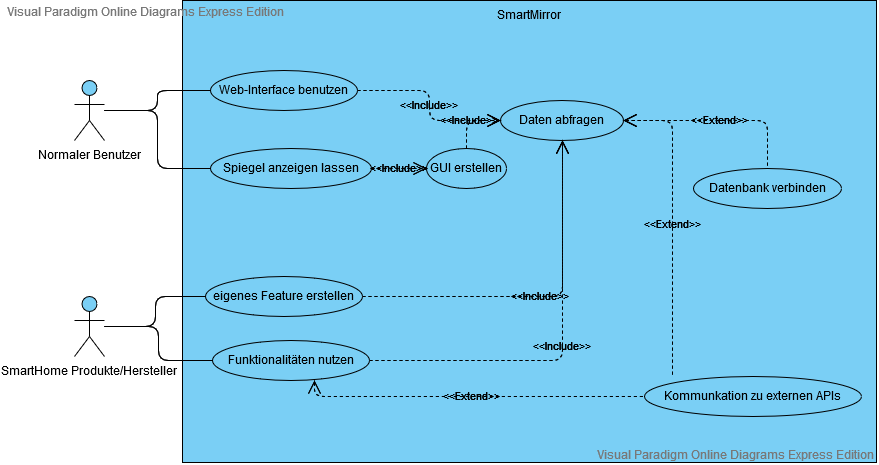
\includegraphics[width=110mm]{pictures/Use-Case-Diagramm.png}
\caption{Use-Case-Diagramm}
\end{figure}
\label{Komponentendiagramm}
\begin{figure}[h]
\centering
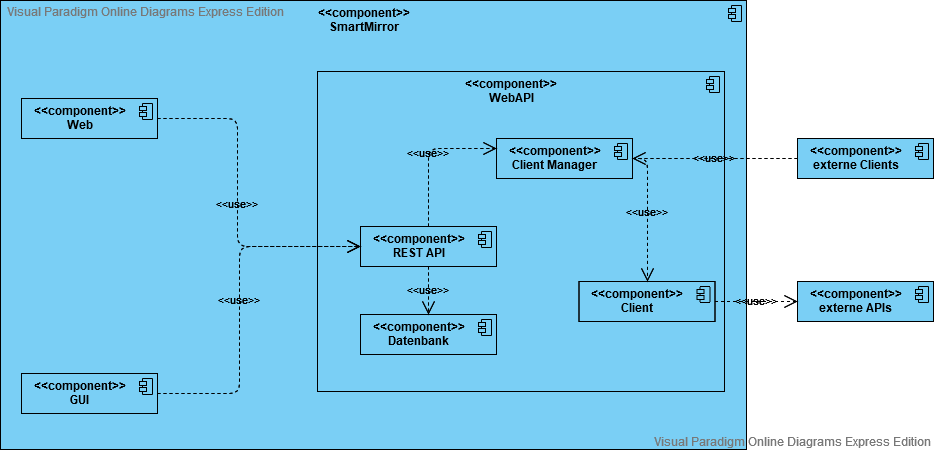
\includegraphics[width=130mm]{pictures/KomponentenDiagramm.png}
\caption{Komponentendiagramm-Diagramm}
\end{figure}
\newpage
\subsection{Verweise}
\subsection{Anmerkungen}

\end{document}